% !TEX root = ../main.tex

\section{\SCXML Translation to \UMLB/\EventB}
\label{sec:translation}

The translation of a specific \SCXML model to \UMLB and  \EventB, comprises the following stages: 
\begin{itemize}
	\item 
Firstly, a basis machine and context are created to embody the semantics of the \SCXML language (as described in Section~\ref{sec:run-completion}).
The basis provides variables and events to model the queue of triggers as well as abstract versions of events to model transitions firing.
The basis is independent of the particular \SCXML model which is added in subsequent refinements.
Hence it is not necessary to re-prove any of the proof obligations associated with this basis.
	\item 
Secondly, all possible combinations of each set of transitions that can fire together are calculated and corresponding events are generated, at appropriate refinement levels (given by the refinement annotations embedded in the \SCXML model), that refine the abstract basis events.
The transitions that can fire together are those that are triggered by the same trigger (or are both untriggered) and are in different parallel (`and') sub-states.
For example, the untriggered transitions shown in the parallel states |FLYOP| and |BATTERYOP| of
figure~\ref{fig:drone4} are combined into an event in the \EventB representation of the model, 
through a conjunction of the guards and actions of each of the transitions. 
If these transitions raise internal triggers, a guard, |{i1, i2, ...} <: content(raisedTriggers)| (where |i1, i2, ...| have been added to the internal triggers set), is introduced to define the raised triggers parameter. 
The subset used in the guard retains non-determinism to allow more triggers to be raised in later refinements.
For triggered transitions, the trigger is specified by a guard that defines the value of the trigger parameter. 
	\item 
Thirdly, at each refinement level, the \SCXML state-chart is translated into a corresponding \UMLB state-machine whose transitions elaborate (i.e., add state change details to) the transition combination events that the transition may be involved in.
A transition may fire in parallel with transitions of parallel nested state-machines that have the same (possibly null) trigger.
	\item
Finally the \UMLB state-machine is translated into \EVENTB by programmatically invoking the \UMLB translator.
\end{itemize}

% Further details of the translation are given in~\cite{MoSn16,MoSnHo18,MoSnHo-ABZ2020}.

 A previous version of the translator was described in~\cite{MoSnHo18,detect2020} New features of the translation added since~\cite{MoSnHo18,detect2020} are as follows:
 \begin{description}
 \item[Trigger queues in basis:]
 	\begin{sloppypar}
 		The encoding of trigger queues in the abstract basis context and machine has been improved so that a queue is properly modelled as a sequence of triggers.
 		This more accurately reflects the \SCXML semantics.
 	\end{sloppypar}
 \item[Dequeing triggers from queues:]
   \begin{sloppypar}
     The abstract basis machine has been improved so that triggers are properly dequeued before potential use,
     which allows triggers to be discarded if the controller cannot respond to them. 
     This more accurately reflects the \SCXML semantics and was necessary in order to model the new drone case study properly.
   \end{sloppypar}

 \item[Finalisation:] Transitions can be flagged as finalised which means their guards can not be strengthened in subsequent refinements. This allows them to `enforced' when they are enabled (i.e., completion cannot occur until they have fired) which is needed for verification. 

 \item[Restricted raising of internal triggers:] Once a trigger is introduced it must immediately be raised at that refinement level by any transitions that wish to do so. It cannot be raised in later refinements except by newly introduced transitions. This restriction was necessary to make simulation more useful by removing non-deterministic raising of triggers in anticipation of refinements.

 \item[Context instantiation:] The axioms of the basis context, that allow future triggers to be added, has been improved so that \PROB\footnote{ProB is an animator, constraint solver and model checker for the B-Method. https://www3.hhu.de/stups/prob} can automatically create an instantiation. 

 \end{description}

A tool to automatically translate \SCXML source models into \UMLB has been produced. 
The tool is based on the \EMF and uses an \SCXML meta-model provided by Sirius~\cite{siriuswebsite} which has good support for extensibility. 
The \UMLB state-machine is subsequently translated into \EVENTB using the standard \UMLB translation which provides variables to model the current state and guards and actions to model the state changes that transitions perform.
% Further details of the translation are given in~\cite{MoSnHo18,MoSnHo-ABZ2020}.

Figure~\ref{fig:drone2UMLB} shows the UML-B model of the drone at refinement level 2 (equivalent to Figure \ref{fig:drone4} without the detail inside TAKEOFF).
The structure of the state-machine is similar to the \SCXML version with purple shading indicating the previously added states and light blue shading indicating the detail added at this refinement level.
State invariants (properties that should hold while that state is active) are shown in |TAKEOFF|, |FLY| and |BATTERYOK|.
Verification of these invariants is discussed in Section~\ref{sec:verificationSafety}.

\begin{figure}[]
%	\vspace{-.4cm}
	\centering
	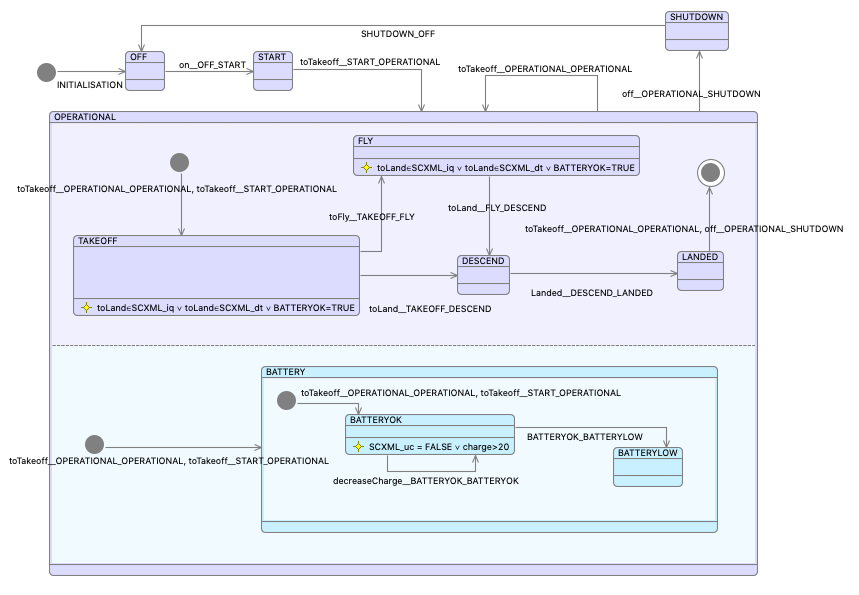
\includegraphics[width=0.90\textwidth, trim=0 40 0 0]{figures/drone2UMLB.png}
	\caption{Generated UML-B State-machine for drone refinement level 2. }
	\label{fig:drone2UMLB}
%	\vspace{-.4cm}
\end{figure} 

%%% Local Variables:
%%% mode: latex
%%% TeX-master: "../main"
%%% End: